\chapter{Инструментальный пакет} \label{relWorks}

В данной главе описан разработанный в рамках данной работы  инструментальный пакет (Software Development Kit, SDK) \textbf{YC.SEL.SDK}, предназначенный для разработки различных решений по статическому анализу динамически формируемых выражений. Представлена архитектура разработанного SDK, а также архитектура надстройки \textbf{YC.SEL.SDK.ReSharper}, позволяющей создавать расширения для ReSharper, предоставляющие поддержку встроенных языков. Изложенный выше алгоритм синтаксического анализа реализован в рамках одной из компонент SDK. YC.SEL.SDK и YC.SEL.SDK.ReSharper являются \textbf{платформами} для разработки инструментов статического анализа динамически формируемого кода.

\section{Архитектура}

Практически любой язык программирования может использоваться как встроенный. При этом нет необходимости рассматривать различные языки, достаточно ограничиться диалектами одного языка. Например, существует множество различных диалектов SQL, каждый из которых имеет свои особенности и каждый из которых может оказаться встроенным языком. Внешним языком также может быть любой язык программирования. Трудность заключается в том, что любое из сочетаний внешнего и встроенного языка может встретиться на практике, и задачи, которые необходимо решать в этой ситуации, могут быть различными (поиск ошибок, подсчёт метрик, автоматизация трансформаций и т.д.). Реализовать универсальный инструмент, решающий все задачи для всех языков, не представляется возможным. Более целесообразно создать набор инструментов, упрощающий создание конечных решений для конкретных языков и конкретных задач. В качестве примера можно рассмотреть инструменты для разработки компиляторов, которые включают в себя генераторы лексических, синтаксических анализаторов и набор библиотек с вспомогательными функциями, и тем самым упрощают создание конкретного компилятора для выбранного языка и целевой платформы.

Требуемый набор инструментов для работы со встроенными языками должен поддерживать весь процесс обработки кода, который может выглядеть так, как представлено на рисунке~\ref{fig:SeqSelProcessing}. Можно выделить следующие основные шаги.
\begin{itemize}
    \item Анализ основного кода, который выполняется сторонним инструментом. Результат этого шага --- это дерево разбора с информацией, достаточной для выполнения дальнейших шагов.
    \item Построение аппроксимации множества возможных значений динамически формируемых выражений.
    \item Лексический анализ построенной на предыдущем шаге аппроксимации.
    \item Синтаксический анализ, результатом которого является лес разбора, пригодный для дальнейшей обработки.
    \item Обработка леса разбора, вычисление семантики.
\end{itemize}

На каждом шаге может быть получена информация, полезная для пользователя, такая как список ошибок, и её необходимо отобразить для него соответствующим образом.

\begin{figure}[h!]
\begin{center}
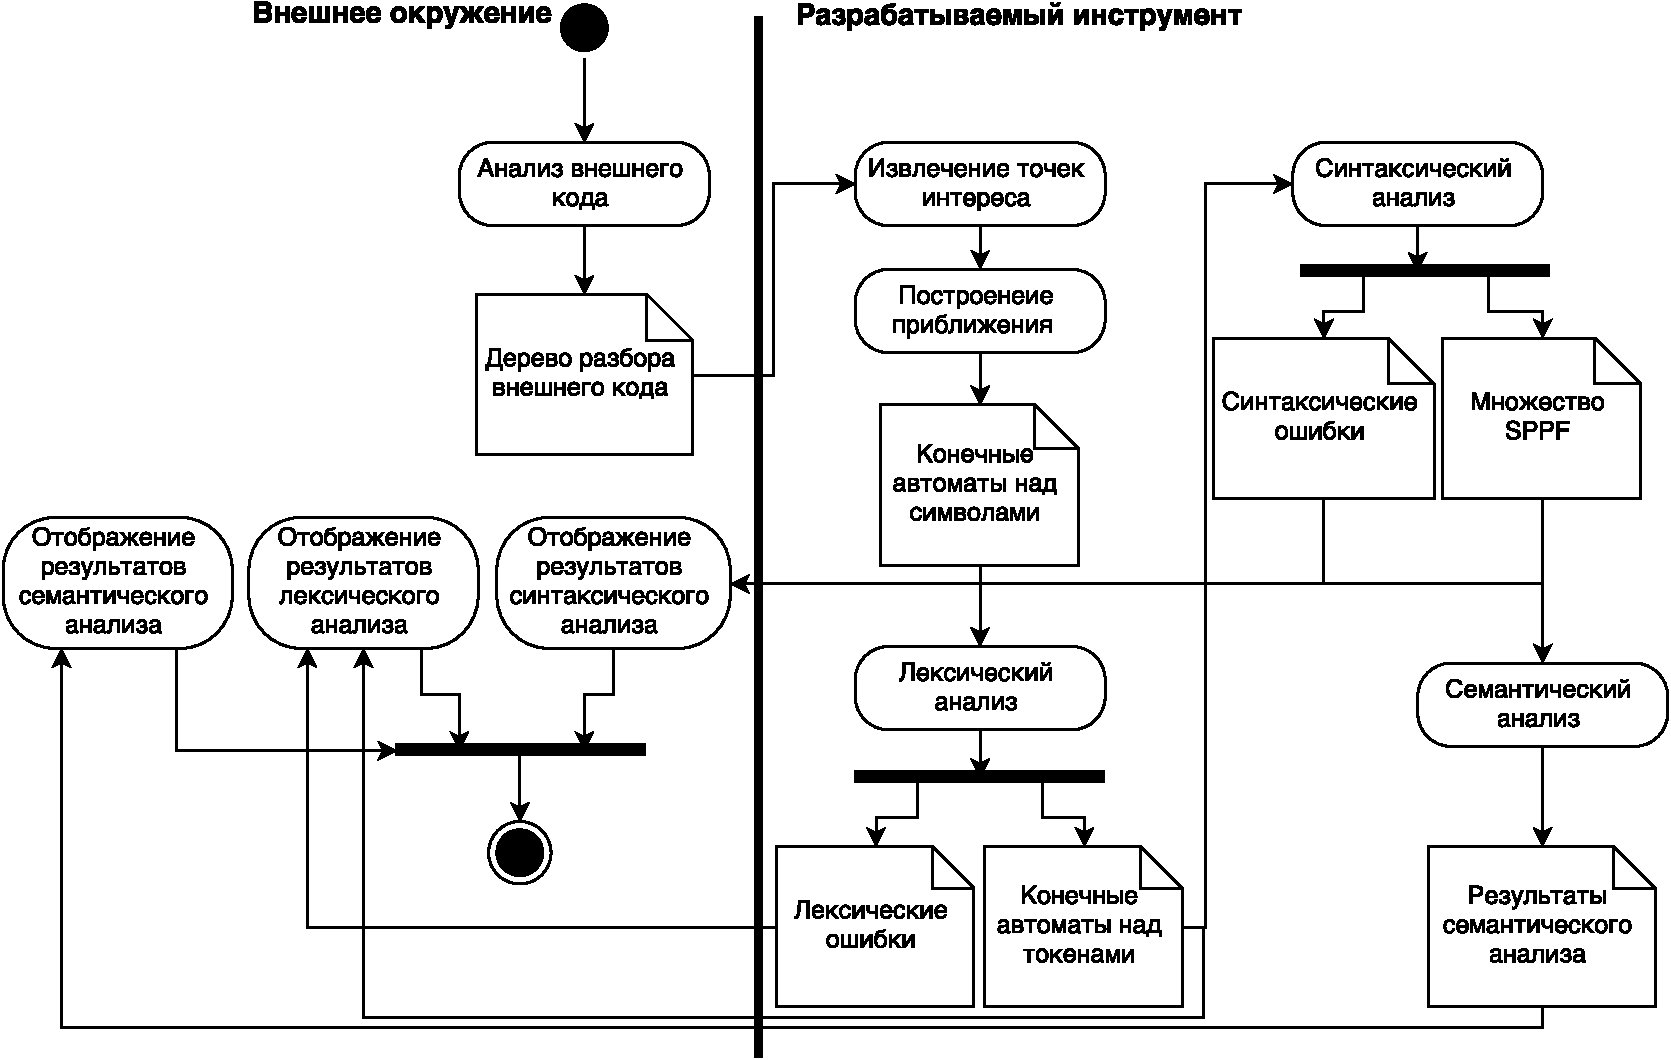
\includegraphics[width=0.9\textwidth]{pics/Activ_SEL_Processing}
\caption{Диаграмма последовательности обработки встроенных языков}
\label{fig:SeqSelProcessing} 
\end{center}
\end{figure}


Существующие инструменты для работы со встроенными языками обычно реализуют поддержку какого-то фиксированного набора языков. При этом поддержка нового языка, как правило, требует нетривиальный доработки инструмента. Чтобы получить поддержку встроенного языка без изменений в исходном коде базового инструмента, необходимо предоставить соответствующий механизм. 

Для того чтобы упростить процесс создания конечных инструментов, создан SDK, одной из компонент которого является генератор синтаксических анализаторов на основе предложенного в данной работе алгоритма. Также в него входит генератор лексических анализаторов, библиотека построения регулярной аппроксимации, набор вспомогательных функций. Подробное описание компонент приведено далее.

Так как анализ внешнего языка является сложной самостоятельной задачей, то он не включён в разработанный SDK. На вход созданному на основе SDK инструменту должно подаваться дерево разбора внешнего языка с информацией, достаточной для решения поставленных в данной работе задач. 


\subsection{Архитектура YS.SEL.SDK}

Разработанный SDK включает компоненты, необходимые для реализации шагов, представленных на рисунке ~\ref{fig:SeqSelProcessing} и описанных ранее, за исключением анализа внешнего языка. Архитектура SDK изображена на рисунке~\ref{fig:SDKHLArch} и включает в себя генераторы анализаторов и различные библиотеки времени исполнения.

\begin{figure}[h!]
\begin{center}
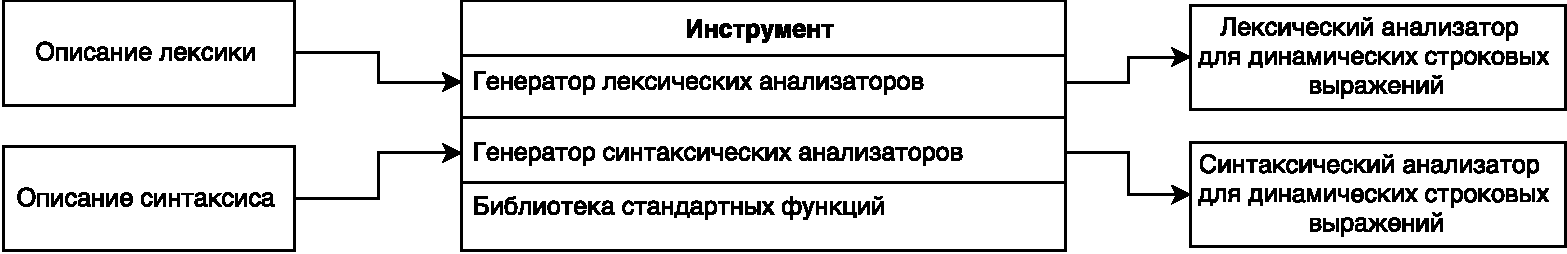
\includegraphics[width=0.9\textwidth]{pics/HighLevelArch}
\caption{Архитектура SDK целиком}
\label{fig:SDKHLArch} 
\end{center}
\end{figure}

Так как анализ внешнего языка не входит в задачи разработанного SDK, то первый шаг, выполнение которого необходимо обеспечить, --- это построение аппроксимации. В нашем случае строится регулярное приближение множества значений динамически формируемого выражения.

Построение регулярной аппроксимации основано на алгоритме, изложенном в работе~\cite{RegOverApprox}, который позволяет строить приближение сверху для множества значений выражений. То есть $L_R$, задаваемый регулярным приближением, не меньше, чем $L_1$, задаваемый программой (выполняется включение $L_R \in L_1$). Это позволяет говорить о надёжности дальнейших анализов в том смысле, что они не теряют информации о $L_1$. Например, это важно при поиске ошибок. Если в $L_R$ не обнаружено ошибок (то есть $L_R \in L_2$, где $L_2$ --- эталонный), значит и в $L_1$ ошибок нет. При этом могут быть найдены ошибки в $L_R$, которых нет в $L_1$, то есть будут ложные срабатывания. Однако наличие ложных срабатываний лучше, чем пропущенные ошибки, и их количество может быть уменьшено путём повышения точности аппроксимации. 

Для того чтобы сделать построение приближения независимым от внешнего языка, реализовано обобщённое представление графа потока управления (Control Flow Graph, CFG)~\cite{Dragon}, которое содержит всю необходимую для дальнейшей работы информацию. Таким образом, разработчику необходимо реализовать построение обобщённого представления CFG для конкретного внешнего языка. В результате компонента строит конечный автомат, являющийся приближением множества значений динамически формируемых выражений.

Архитектура компоненты, отвечающей за лексический анализ, представлена на рисунке~\ref{fig:LexArch}. Основой является  лексический анализатор, который состоит из двух частей: генератора лексических анализаторов, который по описанию лексики обрабатываемого языка, задаваемой в виде файла с расширением fsl (Lexer.fsl), строит соответствующий конечный преобразователь, и интерпретатора, который производит анализ входной структуры данных на основе построенного генератором преобразователя. Конечный преобразователь, построенный по входной спецификации, описывается с виде кода на языке F\# и сохраняется в файле (Lexer.fs). Далее данный файл может быть использован в пользовательском приложении, в рамках которого разрабатывается лексический анализатор, который устроен следующим образом. На вход принимается конечный автомат над символами, результатом работы является конечный автомат над алфавитом токенов анализируемого языка, полученный с помощью интерпретатора и преобразователя, построенного генератором. Входной конечный автомат может быть построен с помощью компоненты построения регулярной аппроксимации. Основные структуры данных --- конечный автомат и конечный преобразователь --- и функции работы с ними описаны в соответствующей библиотеке.

\begin{figure}[h!]
\begin{center}
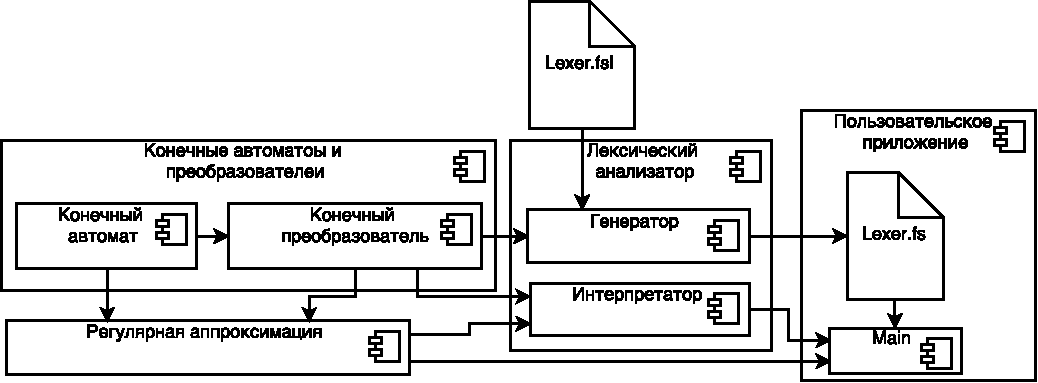
\includegraphics[width=0.95\textwidth]{pics/LexerDiagram}
\caption{Архитектура лексического анализатора}
\label{fig:LexArch} 
\end{center}
\end{figure}

Лексический анализатор реализован на основе инструмента FsLex, который является стандартным генератором лексических анализаторов для языка F\#. При реализации был переиспользован язык описания лексики и некоторые структуры данных.

Реализованный генератор лексических анализаторов обладает следующими особенностями.
\begin{itemize}
    \item Поддерживаются разрывные токены, то есть токены формируемые из нескольких строковых литералов.
    \item Сохраняется привязка лексических единиц к исходному коду: сохраняется информация о строковом литерале, из которого породился токен и координаты его внутри этой строки. Так как одна лексическая единица может формироваться из нескольких строковых литералов, то привязка сохраняется отдельно для каждой части.
    \item Поддерживается обработка входных конечных автоматов, содержащих циклы.
    \item Так как значение токена может формироваться с помощью цикла и, как следствие, быть бесконечным, то каждый токен содержит конечный автомат, порождающий все возможные значения для данного токена, а не единственное значение, как это реализовано в классическом лексическом анализе.
\end{itemize}

\textbf{Генератор синтаксических анализаторов}, названный ARNGLR, реализован на основе алгоритма, описанного в разделе~\ref{AlgoDescr}. Его архитектура представлена на рисунке~\ref{fig:ParsArch}.  

\begin{figure}[h!]
\begin{center}
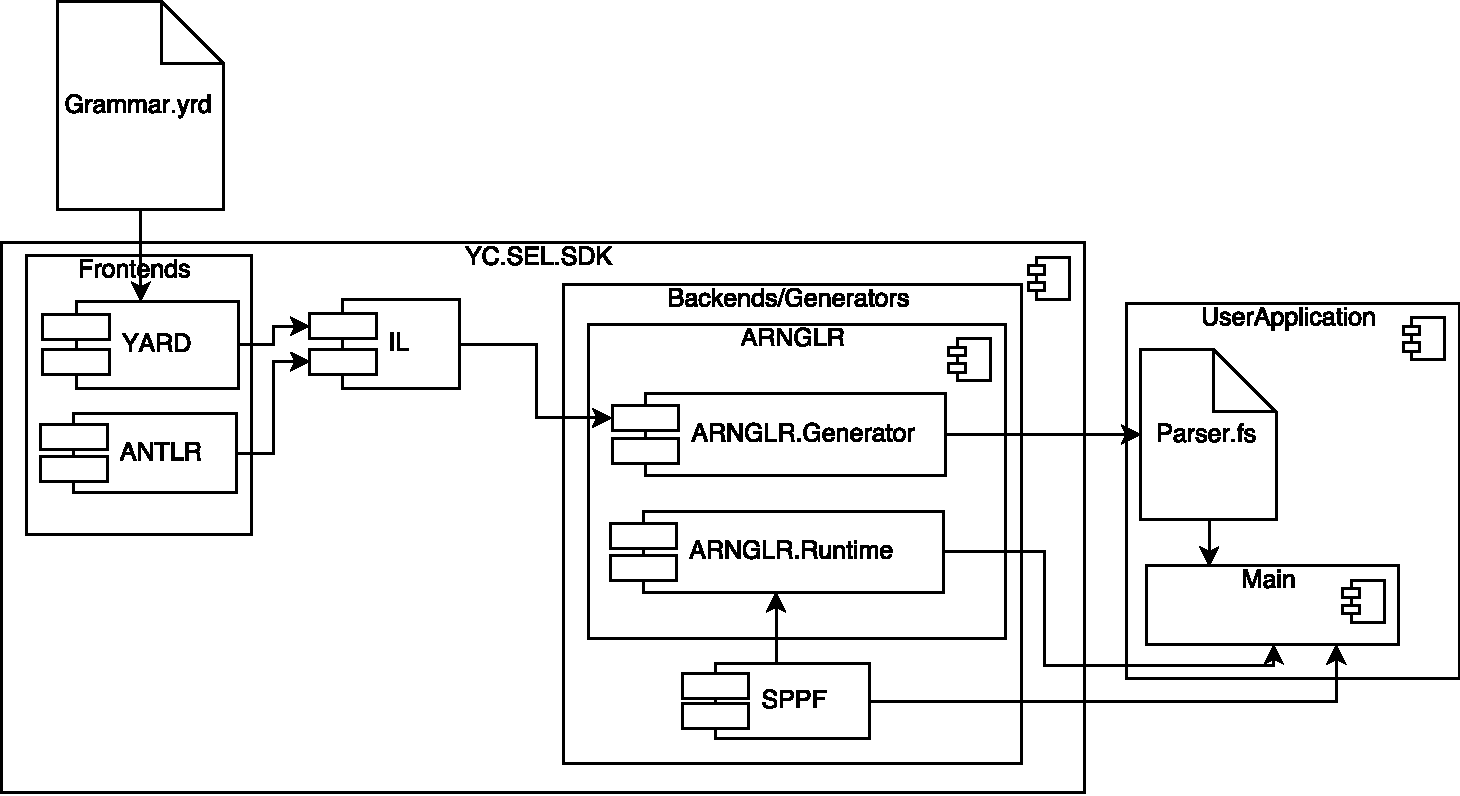
\includegraphics[width=0.95\textwidth]{pics/ARNGLRArch}
\caption{Архитектура синтаксического анализатора}
\label{fig:ParsArch} 
\end{center}
\end{figure}

Генератор реализован как один из модулей YC и может принимать на вход внутреннее представление грамматики (IL), которое может быть получено с помощью различных фронтендов (Frontends), однако в рамках YC.SEL.SDK 
основным фронтендом является YARD, так как он предоставляет наиболее развитые средства для описания грамматик. По грамматике обрабатываемого языка строятся управляющие таблицы анализатора, которые сохраняются в файле Parser.fs. 
Построенные таблицы должны быть включены в разрабатываемое приложение UserApplication. Интерпретатор, предназначенный для синтаксического разбора конечного автомата, полученный после лексического анализа, реализован 
в виде отдельной библиотеки ARNGLR.Runtime, которая также должна быть подключена к разрабатываемому приложению. В результате работы интерпретатора будет получен SPPF, который может быть использован для дальнейшей 
обработки (например, подсчёта метрик). Для упрощения работы с SPPF реализован ряд вспомогательных функций.

\subsection{Архитектура YC.SEL.SDK.ReSharper}

ReSharper --- это расширение к Microsoft Visual Studio IDE, предоставляющее широкий спектр  дополнительной функциональности по анализу и рефакторингу кода. ReSharper поддерживает несколько языков, например C\#, Visual Basic .NET, JavaScript, и этот список может быть расширен благодаря наличию свободно распространяемого ReSharper SDK, описание которого было представлено ранее в разделе~\ref{ReSharperSDKDescr}. ReSharper.SDK позволяет получить деревья разбора для поддерживаемых языков, предоставляет набор готовых анализов и упрощает взаимодействие с Microsoft Visual Studio IDE и её компонентами. Более того, предоставляется возможность разработки собственных расширений для ReSharper на основе ReSharper.SDK.

Microsoft Visual Studio является достаточно распространённой средой разработки, но не поддерживает встроенные языки, поэтому было решено разработать ряд расширений к ReSharper с использованием разработанного инструментария, которые будут устранять данный недостаток. Стоит отметить, что не ставилось задачи поддержать все встроенные языки, так как встроенным может быть любой язык программирования. Также не было необходимости поддержать все внешние языки программирования. Необходимо на базе разработанного YC.SEL.SDK создать инфраструктуру, позволяющую реализовывать поддержку новых встроенных языков в Microsoft Visual Studio через расширения к ReSharper и реализовать несколько расширений, демонстрирующих возможности созданной инфраструктуры. 

Так как необходимо поддерживать различные языки, то необходимо обеспечить расширяемость по новыми языками. Классический подход к решению такой задачи для интегрированных сред разработки заключается в том, что поддержка нового языка реализуется в виде независимой компоненты. Если пользователь хочет получить поддержку какого-либо языка в своей среде разработки, то он должен установить соответствующий пакет. При этом поддержка различных языков осуществляется независимо, однако часто выделяется общая функциональность, которая может быть оформлена в виде отдельного пакета.

Для предоставления описанных выше возможностей была реализована надстройка над YC.SEL.SDK, упрощающая создание расширений для ReSharper, названная  YC.SEL.SDK.ReSharper. В неё включены компоненты, реализующие функции, которые упрощают взаимодействие YC.SEL.SDK и ReSharper.SDK. Назначение основных из них описаны ниже.

\begin{itemize}
  \item Общая точка расширения, необходимая для подключения функциональности для различных встроенных языков, которая может быть реализована в различных расширениях, к ReSharper через общий интерфейс. Также общая точка расширения позволяет использовать общую функциональность, необходимую для работы со встроенными языками.
  \item Отображение в IDE информации, полученной в ходе анализа. Например, подсветка синтаксиса и ошибок. Вывод диагностических сообщений с информацией об ошибках.
  \item Преобразование данных, из формата, используемого в ReSharper.SDK, в формат для YC.SEL.SDK. Например, преобразование графа потока управления внешнего языка, построенного ReSharper.SDK, в формат, пригодный для построения регулярной аппроксимации средствами YC.SEL.SDK.
  \item Управление работой анализаторов, необходимое, с одной стороны, для обеспечения своевременной реакции на изменения в коде, совершённые пользователем, а с другой, для прекращения вычислений, результаты которых уже не актуальны. Управление построено на основе общего для ReSharper механизма, обеспечивающего асинхронную работу анализов. При этом вычисления могут быть прерваны, если, например, пользователь внёс в код изменения, делающие анализ или его результаты некорректными. 
\end{itemize}

Как уже говорилось, встроенными могут быть различные языки и учесть заранее все их особенности не представляется возможным. Кроме того, даже при использовании одного встроенного языка могут использоваться различные способы выполнения сформированного запроса. Таким образом, необходимо предоставлять возможность настройки расширений конечным пользователем. Для этого в рамках YC.SEL.SDK.ReSharper была реализована возможность управления следующими основными параметрами расширений. 

\begin{itemize}
    \item Подсветка синтаксиса для каждого языка. Предоставлена возможность указать цвет для каждого типа токена.
    \item Указание парных элементов. Для каждого языка можно указать, какие лексические единицы считать парными: для каждой пары указывается ``левый'' (открывающая скобка) и ``правый'' (закрывающая скобка) элементы. При расположении курсора в тексте рядом с одним из элементов пары будут подсвечены соответствующие элементы. Пример подсветки парных элементов приведён на рисунке~\ref{fig:braces}.
    \item Точки интереса или хотспоты (hotspot) --- это места, в которых должно быть сформировано финальное выражение. Необходимо знать, какой хотспот какому языку соответствует. При этом нужно учитывать, что одному языку может соответствовать несколько хотспотов. Например, динамически сформированный SQL-запрос в программе на языке программирования C\# может быть выполнен с помощью метода \verb|ExecuteQuery| класса \verb|DataContext|~\cite{ExecuteQuery}
     или же текст запроса может быть передан как аргумент конструктора класса \verb|SqlCommand|~\cite{SqlCommand} с последующим выполнением с помощью метода \verb|ExecuteReader|.

\end{itemize}

Настройка указанных выше параметров хранится в соответствующих конфигурационных файлах в формате XML, которые на данный момент редактируются вручную. Настройка подсветки синтаксиса и парных элементов совмещена в одном файле и для каждого языка создаётся отдельный такой файл. Конфигурационный файл с точками интереса является общим для всех языков и, соответственно, для всех установленных расширений для поддержки встроенных языков.

В листинге~\ref{lst:codeHighlighting} приведён пример конфигурации подсветки синтаксиса и парных скобок для языка Calc. Для указания цвета используются имена, принятые в ReSharper (например, \verb|"CONSTANT_IDENTIFIER_ATTRIBUTE"|), что должно сделать настройку цветов более единообразной. В xml-тэге \verb|Matched| содержится описание парных элементов. Каждая пара описывается в xml-тэге \verb|Pair| и для одного языка может быть указано более одной такой пары.

\fvset{frame=lines,framesep=5pt}
\begin{listing}[H]
    \begin{pyglist}[language=xml,numbers=left,numbersep=5pt]
<?xml version="1.0" encoding="utf-8"?>
<SyntaxDefinition name="CalcHighlighting">
    <Colors>
        <Tokens color="CONSTANT_IDENTIFIER_ATTRIBUTE">
            <Token> DIV </Token>
            <Token> LBRACE </Token>
            <Token> MINUS </Token>
            <Token> MULT </Token>
            <Token> NUMBER </Token>
            <Token> PLUS </Token>
            <Token> POW </Token>
            <Token> RBRACE </Token>
        </Tokens>
    </Colors>
<!-- Dynamic highlighting: -->
    <Matched>
        <Pair>
            <Left> LBRACE </Left>
            <Right> RBRACE </Right>
        </Pair>
<!-- You can specify more then one pair:        
        <Pair>
            <Left> LEFT_SQUARE_BRACKET </Left>
            <Right> RIGHT_SQUARE_BRACKET </Right>
        </Pair>
        <Pair>
            <Left> LEFT_FIGURE_BRACKET </Left>
            <Right> LEFT_FIGURE_BRACKET </Right>
        </Pair>
-->        
    </Matched>
</SyntaxDefinition>
    \end{pyglist}
\caption{Пример конфигурационного файла для настройки подсветки синтаксиса}
\label{lst:codeHighlighting}
\end{listing}

Листинг~\ref{lst:hotspots} содержит пример описания точек интереса. Для каждой точки интереса должна быть указана следующая информация.
\begin{itemize}
    \item Какому встроенному языку соответствует точка. Информация хранится в Xml-тэге \verb|Language|.
    \item Полное имя метода, являющегося точкой интереса. Информация хранится в Xml-тэге \verb|Method|.
    \item Порядковый номер аргумента данного метода, являющегося выражением на встроенном языке. Нумерация начинается с нуля. Информация хранится в Xml-тэге \verb|ArgumentPosition|. 
    \item Возвращаемый тип метода.  Информация хранится в Xml-тэге \verb|ReturnType|. 
\end{itemize}

\fvset{frame=lines,framesep=5pt}
\begin{listing}[H]
    \begin{pyglist}[language=xml,numbers=left,numbersep=5pt]
<?xml version="1.0" encoding="utf-8"?>
<!-- comment about body -->
<Body>
    <!-- comment about hotspot -->
  <Hotspot>
      <!-- comment about tsql -->
      <Language> TSQL </Language>
      <!-- comment about fullName -->
      <Method>Program.ExecuteImmediate</Method>
      <!-- zero-based -->
      <ArgumentPosition> 0 </ArgumentPosition>
      <!-- comment about return type -->
      <ReturnType> void </ReturnType>
  </Hotspot>
  <Hotspot>
      <Language> Calc </Language>
      <Method>Program.Eval</Method>
      <ArgumentPosition> 0 </ArgumentPosition>
      <ReturnType> int </ReturnType>
  </Hotspot>
</Body>
    \end{pyglist}
\caption{Пример конфигурационного файла для настройки точек интереса}
\label{lst:hotspots}
\end{listing}


\section{Области и способы применения YC.SEL.SDK}

Разработанный SDK предназначен для создания инструментов статического анализа динамически формируемых строковых выражений. Решения, созданные с его помощью, могут применяться для работы с проектами, активно использующими динамически формируемые строковые выражения. Необходимость работать с такими проектами может возникнуть, например, в следующих областях.

\begin{itemize}
    \item Реинжиниринг программного обеспечения.
    \item Поддержка встроенных языков в средах разработки.
    \item Оценка качества и сложности кода.
\end{itemize}

Общим для всех этих областей является то, что для решения многих задач необходимо структурное представление динамически формируемого кода. При этом анализируемые языки могут быть различными и процесс их анализа часто тесно связан с анализом внешнего языка.

Отметим, что встроенные языки используются всё менее активно в молодых проектах и системах. На смену им приходят более надёжные способы композиции языков и метапрограммирования. Например LINQ или ORM-технологии. Однако это не всегда так. Использование строковых выражений для взаимодействия с базами данных и генерации WEB-страниц в приложениях на PHP всё ещё широко распространено~\cite{DSQLInActiveUse}. Это необходимо учитывать при поддержке встроенных языков в средах разработки. Для каких-то языков на первый план выходят возможности по изучению и модификации уже созданного кода, а для каких-то --- возможность быстро и удобно создавать новый код. Во втором случае могут возникнуть дополнительные требования к скорости работы инструмента, так как подразумевается выполнение некоторых операций ``на лету'', что может послужить ограничением на использование SDK, так как многие механизмы, реализованные в нём, не предусматривают возможности уменьшения точности в пользу увеличения быстродействия. Оценка качества и сложности  кода часто может выполняться в рамках комплекса задач по реинжинирингу системы, однако может быть и самостоятельной задачей, например, при оценке сложности работ по поддержке и сопровождению информационной системы.

Детали применения SDK могут варьироваться в зависимости от решаемых задач и контекста использования. Например, механизм построения регулярной аппроксимации может быть реализован независимо в рамках внешнего инструмента. Однако основной сценарий использования аналогичен использованию инструментариев для разработки компиляторов. Последовательность шагов, представленная ниже, может быть изменена в зависимости от особенностей задачи.

\textbf{Шаг 1.} Создание грамматики обрабатываемого языка. Грамматика может быть создана на основе документации соответствующего языка или переиспользована готовая, что оправданно, например, при создании анализатора для динамического SQL, когда внешний и встроенный языки совпадают.

\textbf{Шаг 2.} Генерация синтаксического анализатора по созданной грамматике. Для этого используется генератор синтаксических анализаторов, присутствующий в SDK. Результатом работы генератора является файл с исходным кодом на языке программирования F\#, который должен быть включён в разрабатываемый код. Файл содержит описание типов для лексических единиц, управляющие таблицы анализатора и функцию, которая по конечному автомату над алфавитом токенов анализируемого языка построит SPPF, содержащий деревья вывода всех корректных цепочек.

\textbf{Шаг 3.} Создание лексической спецификации обрабатываемого языка. Спецификация может быть извлечена из документации или заимствована из других проектов. При обработке динамически формируемого SQL возможно переиспользовать спецификацию, созданную для основного языка, которым также является SQL. При этом необходимо обратить внимание на то, что типы лексических единиц определяются на основе созданного на предыдущих шагах синтаксического анализатора.

\textbf{Шаг 4.} Генерация лексера по созданной спецификации. Для этого применяется генератор лексических анализаторов, входящий в состав SDK. В результате его применения получается файл с исходным кодом на языке F\#, который должен быть подключён к разрабатываемому решению. 

\textbf{Шаг 5.} Реализация механизма построения регулярной аппроксимации, результатом которого является функция, строящая конечный автомат над алфавитом символов. Данный механизм может быть реализован либо на основе предоставляемого в рамках SDK, либо независимо. В первом случае от разработчика требуется построить обобщённый CFG для внешнего языка. Во втором случае необходимо только гарантировать правильность возвращаемого конечного автомата. Второй подход может быть использован, например, при наличии реализованного механизма протягивания констант для внешнего языка. Это позволит создать возможно менее точное, но, скорее всего, более быстрое построение аппроксимации. Такой подход применим при автоматизированном реинжиниринге, когда ручная доработка кода является обязательным шагом и абсолютная точность автоматической обработки не требуется. Ещё одна возможная область применения второго подхода --- это поддержка встроенных языков в средах разработки. Здесь также часто не требуется высокая точность для подсказок пользователю, однако производительность крайне важна. Поэтому иногда приходится жертвовать точностью анализа для достижения нужной скорости работы.

\textbf{Шаг 6.} Реализация работы с SPPF. Синтаксический анализатор возвращает SPPF --- конечное представление леса разбора всех корректных цепочек из аппроксимации. Дальнейшая работа с ним может строиться по двум основным сценариям.

Первый сценарий --- непосредственная обработка SPPF. В этом случае все вычисления происходят над SPPF без извлечения отдельных деревьев. Это позволит ускорить обработку результатов разбора, так как количество деревьев может быть бесконечным, а SPPF является конечной структурой данных. Однако существует несколько проблем, связанных с таким подходом. Во-первых, требуется создание новых процедур обработки, так как классические, как правило, ориентированы на работу с деревьями. Во-вторых, могут возникнуть трудности при выполнении некоторых анализов, вызванные тем, что в SPPF хранятся ``бесконечные'' деревья. Например, необходимо вычислить максимальную глубину вложенности конструкции \verb|if|, являющуюся одной из стандартных метрик сложности кода. SPPF может содержать 
циклы и может оказаться так, что конструкция \verb|if| встречается в цикле таким образом, что потенциальная глубина вложенности может быть бесконечной. Такая ситуация не является стандартной при 
обработке деревьев разбора и её надо отслеживать отдельно.

Второй сценарий --- извлечение отдельных деревьев из SPPF и их обработка. Данный подход может оказаться удобным, если уже существуют процедуры обработки синтаксических деревьев для языка, который оказался встроенным. Это помогает избежать затрат на создание новой функциональности. Такое может произойти при работе с динамическим SQL. В этом случае для работы с деревом разбора внешнего языка и деревьями, извлечёнными из SPPF, можно использовать одни и те же процедуры, так как языки идентичны.

Недостатком второго подхода является то, что конечность числа деревьев не гарантирована. Это значит, что не удастся обработать все деревья. Стоит отметить, что даже в случае конечности числа деревьев, перебор и обработка всех деревьев разбора может потребовать значительных ресурсов.


\textbf{Шаг 7.} Реализация механизмов сбора, обработки и отображения информации, такой как сообщения об ошибках или любой другой, полученной в процессе анализа. Необходимо для предоставления пользователю информации, ожидаемой в рамках решаемой задачи.

На рисунке~\ref{fig:activMethod} изображён один из возможных сценариев использования SDK. Особенностью является цикличность процесса, характерная, например для реинжиниринга программного обеспечения.

\begin{figure}[h!]
\begin{center}
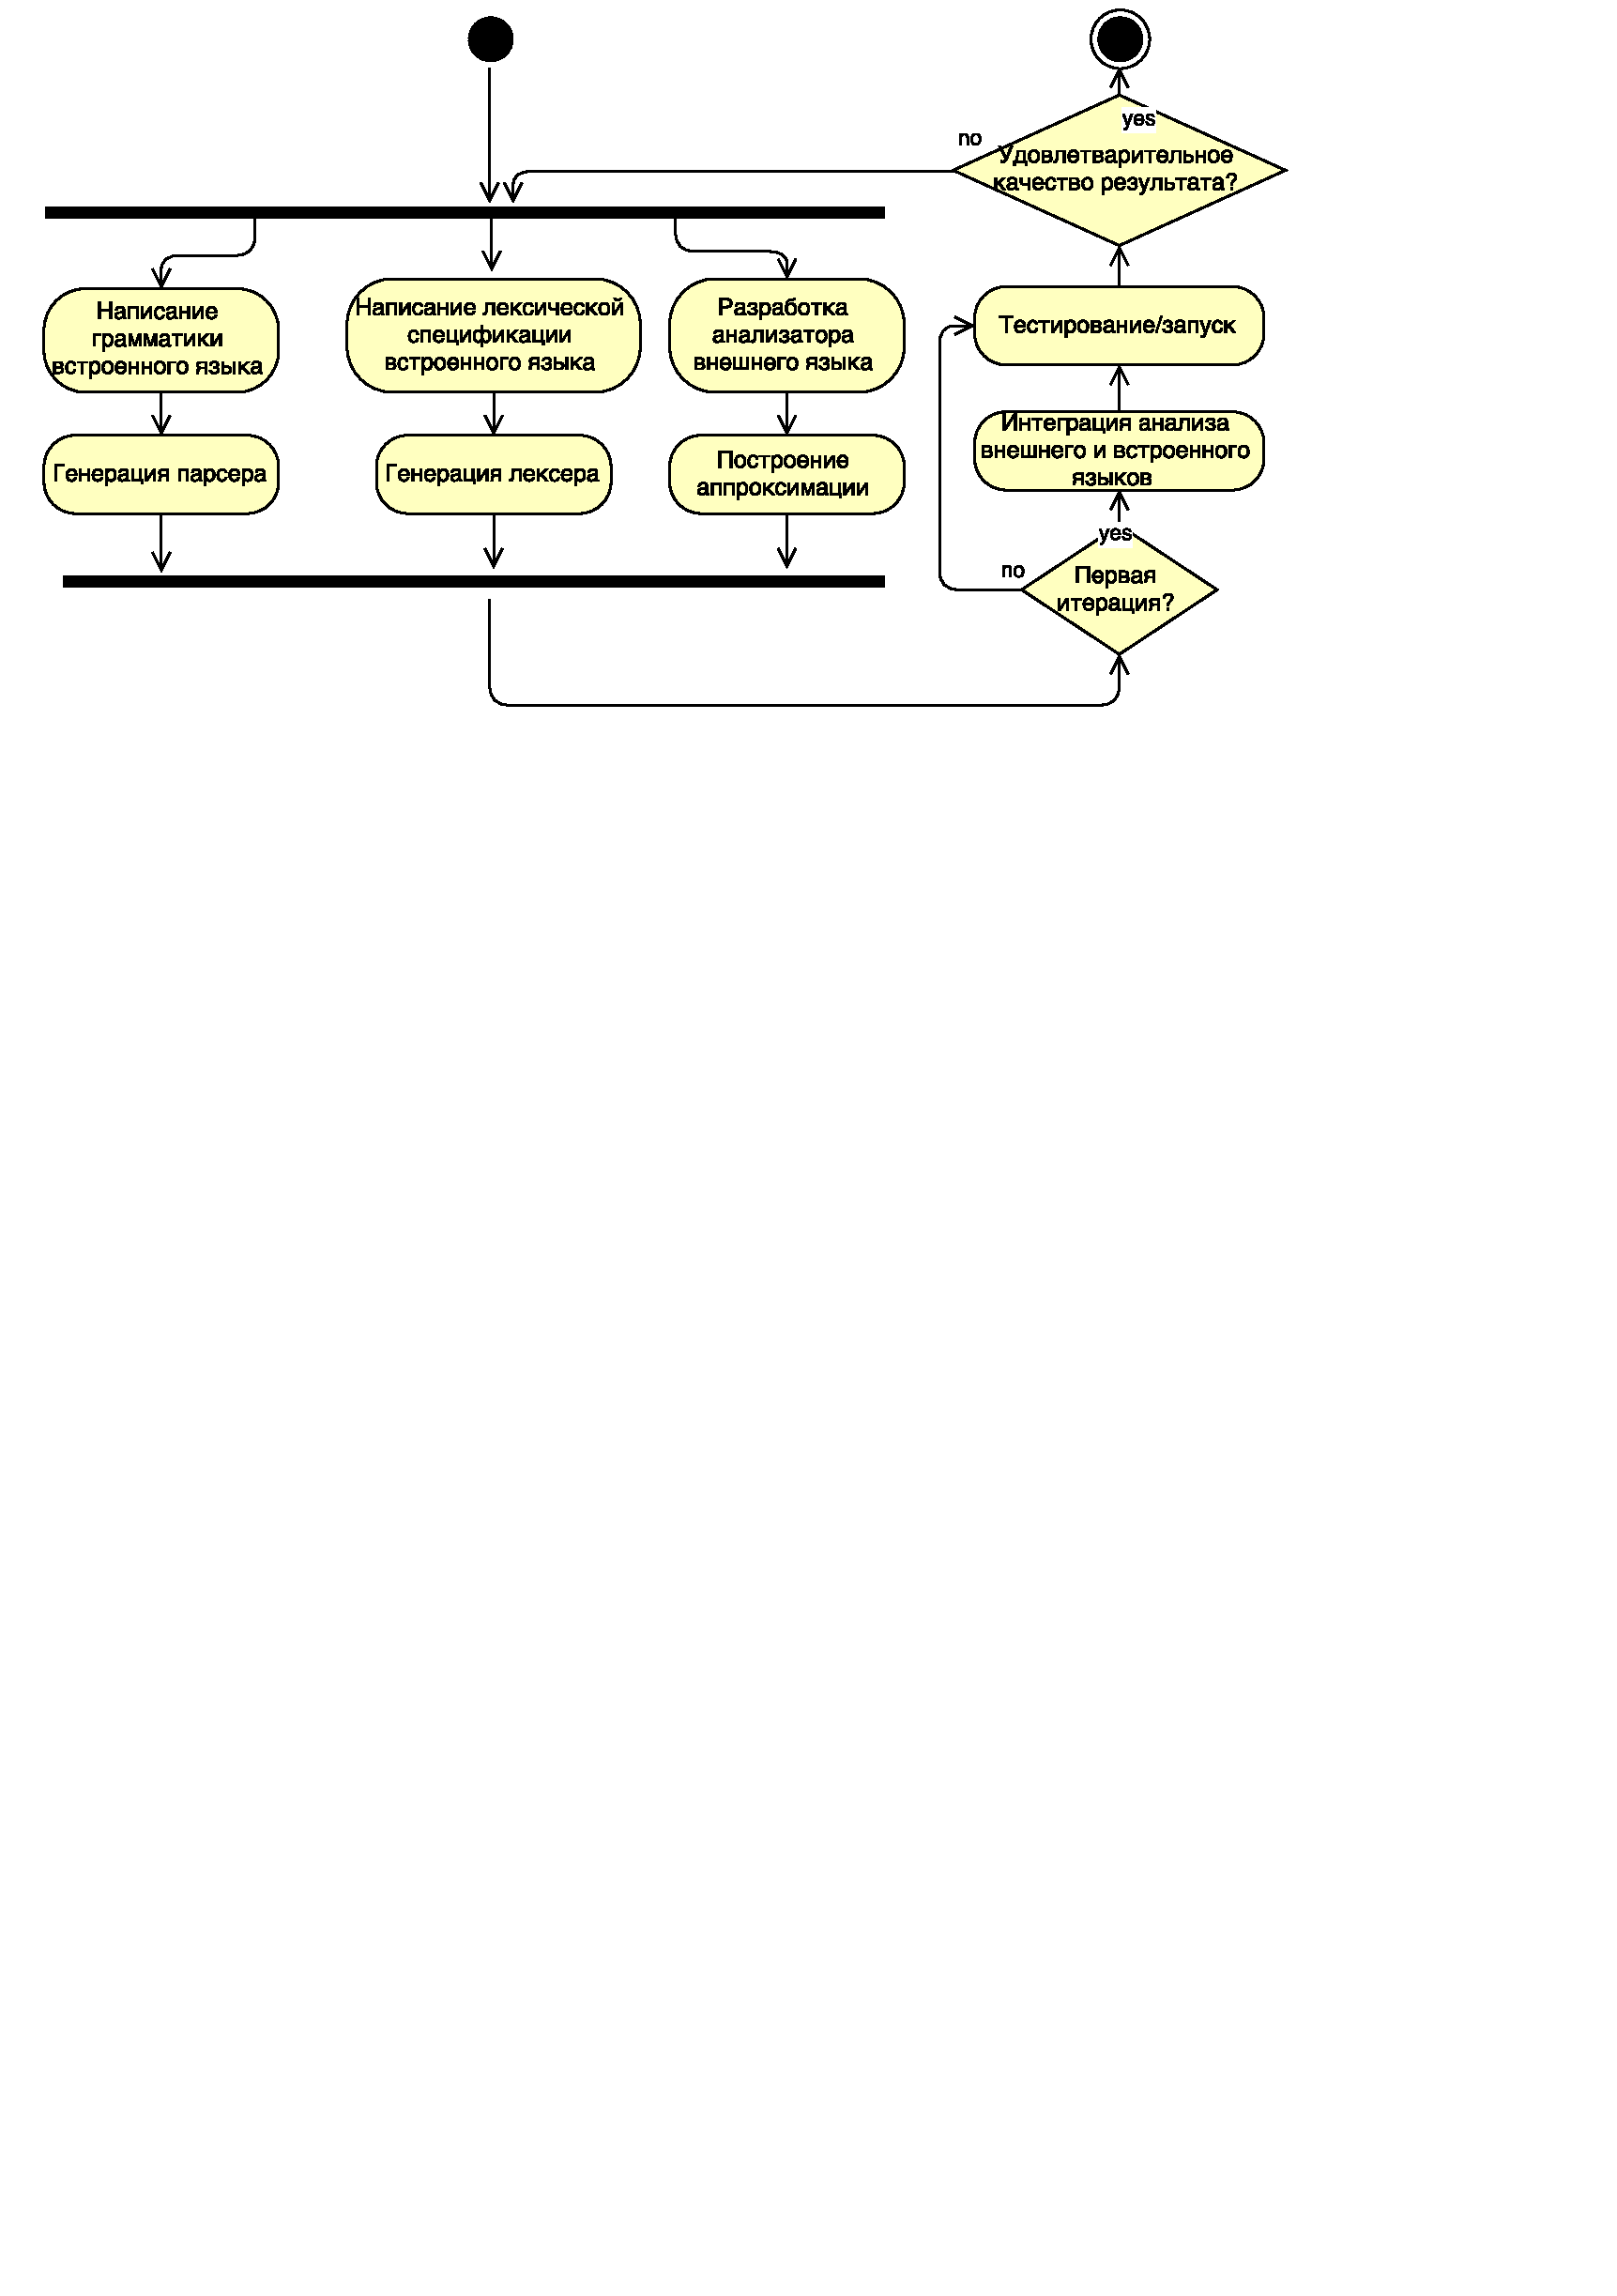
\includegraphics[width=0.9\textwidth]{pics/ActivMethodology}
\caption{Один из возможных вариантов использования SDK в проектах по реинжинирингу}
\label{fig:activMethod} 
\end{center}
\end{figure}

Встраивание анализа строковых выражений в последовательность обработки кода всей системы зависит от решаемых задач. Первыми шагами идут действия, необходимые для того, чтобы получить входные данные для анализа. Для этого необходимо провести лексический и синтаксический анализ внешнего языка, построить граф потока управления. После этого возможно построение аппроксимации и дальнейший анализ встроенных языков. Параллельно с этим может проводиться дальнейшая обработка внешнего языка. Степень параллельности зависит от независимости решаемых задач. Например, некоторые метрики сложности для основного кода и для динамически формируемого можно считать независимо и выводить отдельно. С другой стороны, может возникнуть необходимость вычислить некую комплексную метрику, учитывающую параметры и внешнего и динамически формируемого кода, что приведёт к необходимости синхронизации.

\section{Особенности реализации}

Разработка инструментального пакета с описанной выше архитектурой и плагинов для ReSharper велась в рамках исследовательского проекта YaccConstructor (YC), описанного в разделе~\ref{YCDescr}. 
Разработка велась на платформе .NET и основной язык реализации --- F\#~\cite{FSharp}. Весь исходный код опубликован на GitHub~\cite{YCUrl}. 
Большинство компонент опубликовано под ``открытой'' лицензией Apache License Version~2.0~\cite{ApacheV2}. 

За основу алгоритма синтаксического анализа динамически формируемых выражений был взят реализованный в YC алгоритм синтаксического анализа RNGLR. Генератор управляющих таблиц был использован практически без 
модификаций, а интерпретатор был реализован отдельный. Кроме этого, общими являются некоторые структуры данных и вспомогательные функции, такие как представление леса разбора и его печать в формате 
DOT~\footnote{DOT --- текстовый язык описания графов~\cite{DOT}.}, представление GSS. 

Лексический анализ реализован на основе инструмента FsLex, который потребовал значительных доработок для того, чтобы обеспечить обработку конечного автомата, а не линейного входа. Все остальные компоненты, 
необходимые для статического анализа динамически формируемых выражений, такие как построение аппроксимации, вспомогательные функции для упрощения построения целевых инструментов были реализованы ``с нуля'' 
в рамках проекта YC.

Бинарные пакеты, содержащие основную функциональность, опубликованы в сети интернет на NuGet~\footnote{NuGet --- менеджер пакетов для платформы .NET и одноимённый ресурс для их публикации. Позволяет публиковать 
и устанавливать пакеты, автоматически отслеживать зависимости между ними~\cite{NuGet}.}.
